\documentclass[11pt]{article}
\usepackage{classTools}
\usepackage[normalem]{ulem}
\usepackage{graphicx}
\begin{document}

% To include aws problems set header, use the psHeader command
\psHeader{7}{Wed Nov. 9, 2022 (11:59pm)}

\textbf{Your name: Nikhil Datar}

\textbf{Collaborators: Adam Zhou}

\textbf{No. of late days used on previous psets: 6}

\textbf{No. of late days used after including this pset: }


The purpose of this problem set is to develop skills in implementing graph algorithms, appreciate the impact of different kinds of worst-case exponential algorithms in practice, and practice reducing problems to SAT.
\begin{enumerate}

    \item (Another coloring algorithm) 
  In the \href{https://github.com/Harvard-CS-120/cs120/tree/main/fall2022/psets/ps7}{Github repository for PS7}, we have given you basic data structures for graphs (in adjacency list representation) and colorings, an implementation of the coloring algorithm from ps5, and a variety of test cases (graphs) for coloring algorithms. For Windows users, use this \href{https://colab.research.google.com/drive/13nMhNMaDstVaEkxye61m8AV7nk9ks9uS#scrollTo=AbIalcylVVuu}{Google Colab} file to run your code.
  
  \begin{enumerate}      
      \item Implement the reduction from 3-coloring to SAT given in class in the function \texttt{sat\_3\_coloring}, producing an input that can be fed into the SAT Solver \href{https://pysathq.github.io/usage/}{Glucose}, and verify its correctness by running \texttt{python3 -m ps7\_tests 3}. \label{part:SAT}
      \item Compare the efficiency of Exhaustive-Search 3-coloring, the $O(1.89^n)$-time BFS-based algorithm for 3-coloring from problem set 5 (feel free to use the staff solution or your own implementations from problem set 5), and your implementation from  Part~\ref{part:SAT} using \texttt{ps7\_experiments}. In the experiments file, we've provided code to generate two types of graphs (lines of rings and clusters of independent sets) and some new specific graphs. For each of those types of graphs, how many of the given instances, if any, can each algorithm solve within 10 seconds (same time limit as problem set 5)? You should fill out the table and briefly discuss and try to explain your findings.

\begin{center}
    \begin{tabular}{|c|l|l|l|}
    \hline 
    Algorithm
    & \multicolumn{1}{|p{2cm}|}{Exhaustive}
    & \multicolumn{1}{|p{2cm}|}{ISET BFS}
    & \multicolumn{1}{|p{2cm}|}{SAT Color}\\\hline
    \hline
        \# Solvable Ring Instances  & $0/6$ & $2/6$ & $6/6$\\
        \# Solvable Cluster Instances & $4/6$  & $4/6$ & $6/6$\\
        \# Solvable Other Graphs  & $0/3$ & $0/3$ & $2/3$ \\
        \hline
    \end{tabular}
\end{center} \\

The table above shows that SAT Color was able to solve the most number of ring instances, cluster instances, and other graphs. The ISET BFS algorithm solved the second most number of ring instances, and solved the same number of cluster instances (4/6) and other graphs (0/3) as exhaustive search. These results can be explained by analyzing the runtime of the algorithms. In particular, we know the fastest SAT solvers to be $ \approx O(1.33^{n})$ runtime, whereas the ISET BFS algorithm used we know to be $O(1.89)^n$ and exhaustive to be in the best case for 3-coloring $O(3^n)$ runtime. Additionally, in the reduction from $k$-coloring to the SAT problem, if we treat the oracle call to the SAT solver Glucose3 as $O(1)$, then the runtime of the reduction is $O(n+km)$. Meanwhile, as already mentioned, the Glucose3 solver is still exponential, but much faster than most SAT solvers and the other two algorithms. Although the runtime of the particular SAT solver used (Glucose3) is uncertain, it is clear that it is likely close to the best SAT solvers, since indeed it solved more ring instances, cluster instances, and other graphs than both ISET BFS and Exhaustive algorithm. Additionally, we did see ISET BFS solve more ring instances than Exhaustive, which makes sense since the runtime is faster.

    \item (optional\footnote{This problem is meant to be done based on your enjoyment/interest and only if you have time. It won't make a difference between N, L, R-, and R grades, and course staff will deprioritize questions about this problem at office hours and on Ed.}) Find a graph $G$ such that Glucose takes more than 1 second to solve the SAT instance to which the 3-colorability of $G$ was reduced in part a, and $n$ is as small as you can make it. Describe your approach to finding such a $G$. 
  \end{enumerate}

\item (Resolution) Use the algorithm \texttt{ResolutionInOrder} that we saw in Lecture 16 to decide the satisfiability of the following formulas, and use the algorithm \texttt{ExtractAssignment} to obtain a satisfying assignment for any that are satisfiable. (Please make sure to follow both algorithms \textit{exactly}, including the order in which the clauses are processed. A correct final solution that does not show all of the intermediate steps of both algorithms will not receive full score.)
  
  \begin{enumerate}
      \item $\varphi(x_0, x_1, x_2, x_3) = (x_2 \vee \neg x_1) \wedge (x_3 \vee x_1) \wedge (x_0 \vee x_1) \wedge (\neg x_3) \wedge (\neg x_1 \vee \neg x_2)$. \\
      
      We define the clauses from above. $C_0 = (x_2 \vee \neg x_1)$, $C_1 = (x_3 \vee x_1)$, $C_2 = (x_0 \vee x_1)$, $C_3 = (\neg x_3)$, $C_4 = (\neg x_1 \vee \neg x_2)$. Then, we start the ResolutionInOrder process. Within the following images, we denote $\neg$ with the $-$ sign.
      
      Now the work for ResolutionInOrder is shown below. \\
      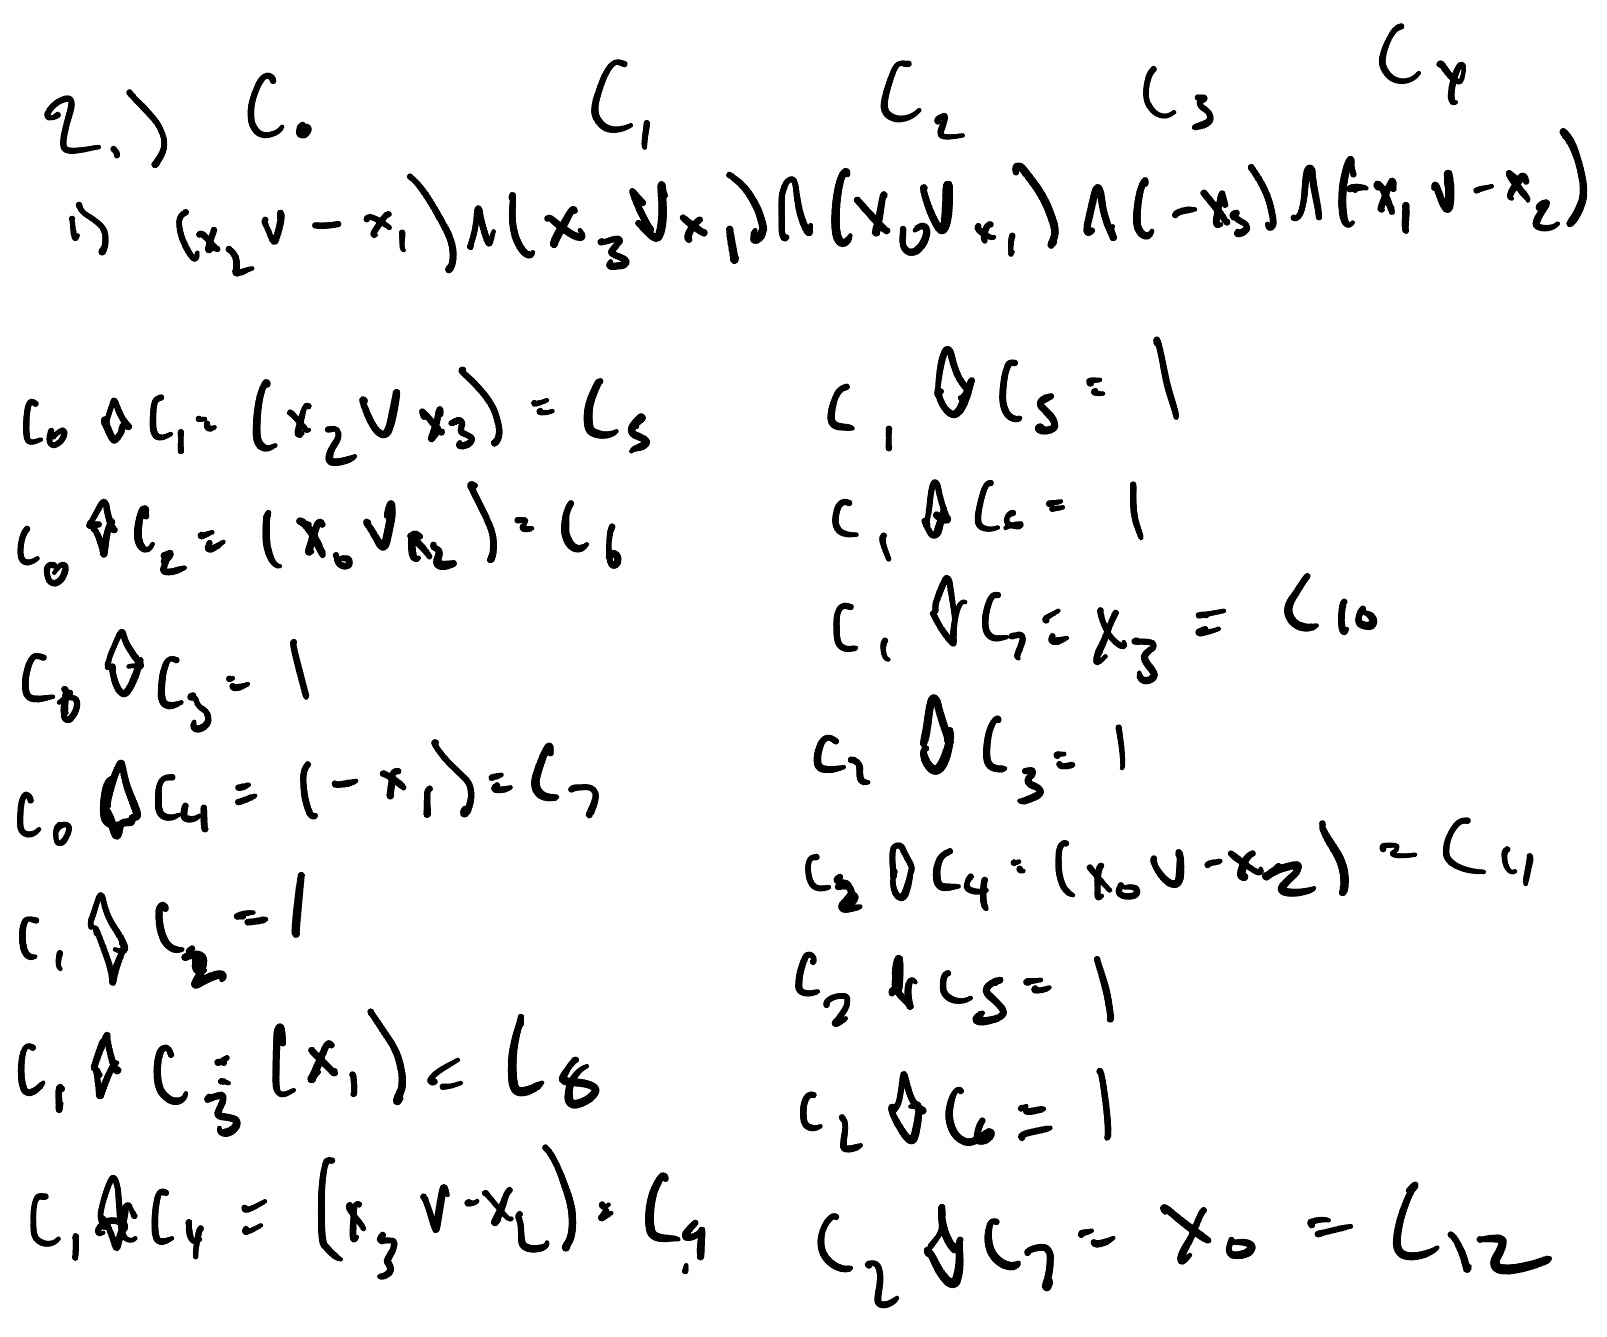
\includegraphics[width=.6\textwidth]{fall2022/psets/ps7/IMG_0015.jpg} \\
      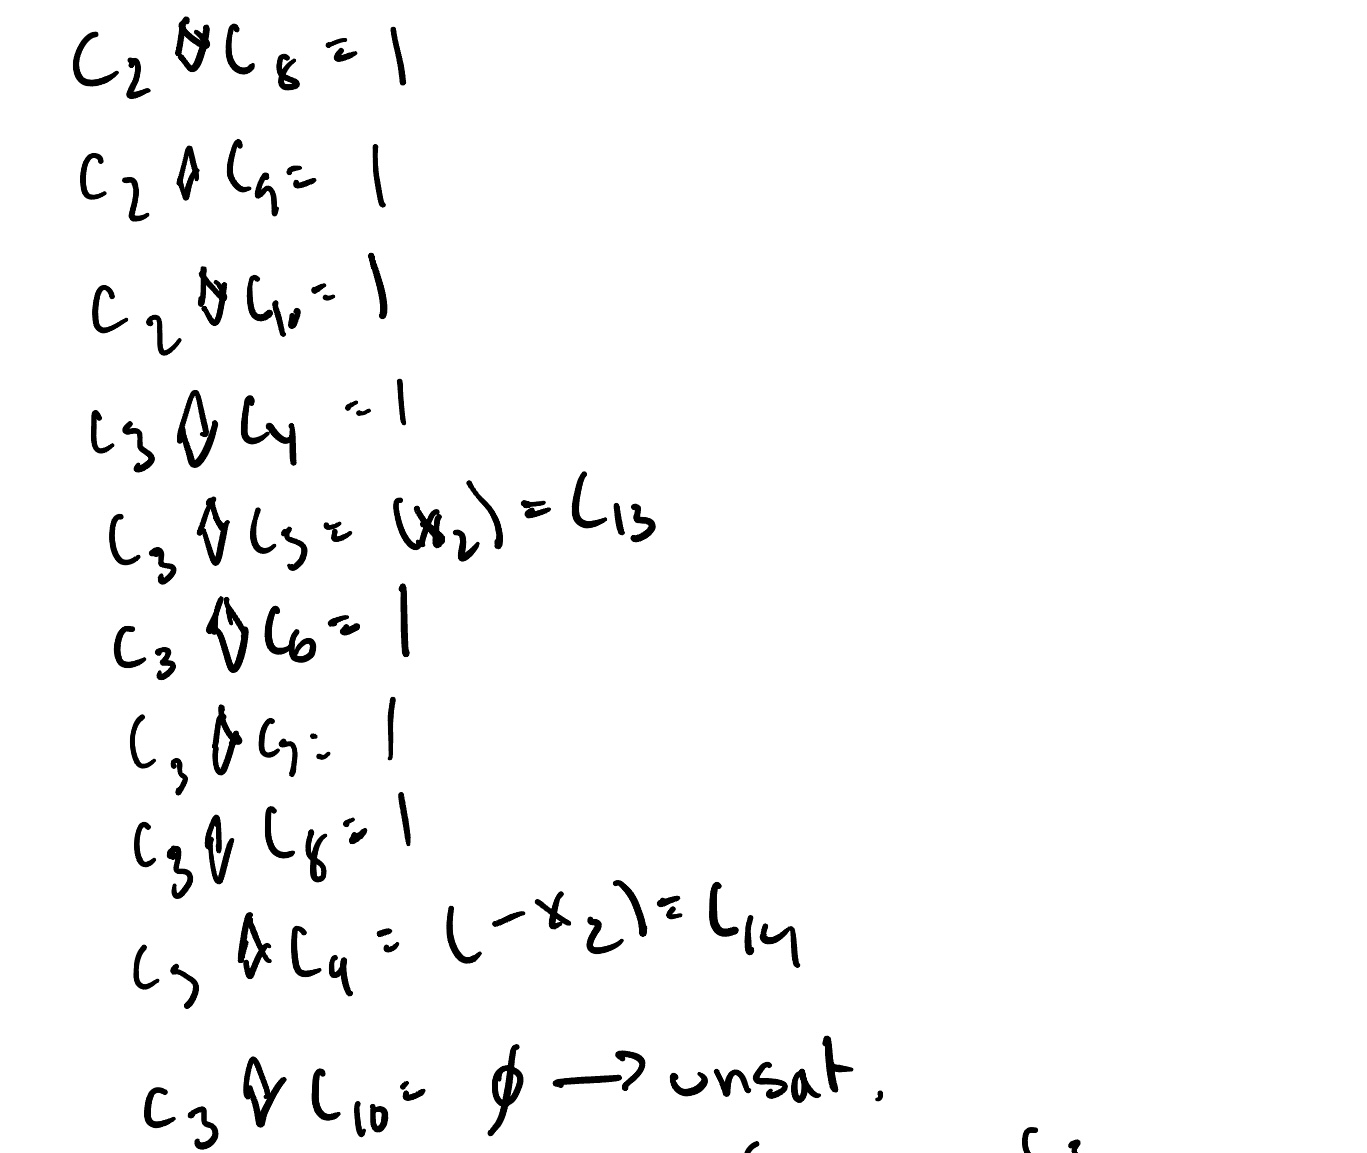
\includegraphics[width=.6\textwidth]{fall2022/psets/ps7/IMG_0016.jpg} \\
      
      Thus the problem is unsatisfiable. 

      \item $\varphi(x_0, x_1, x_2) = (x_0) \wedge (\neg x_0 \vee x_1) \wedge (\neg x_1 \vee \neg x_2) \wedge (x_2)$.\\
      
      We start similarly like part a defining clauses. We have $C_0 = (x_0)$, $C_1 = (\neg x_0 \vee x_1)$, $C_2 = (\neg x_1 \vee \neg x_2)$, $C_3 = (x_2)$. Then, we continue with ResolutionInOrder. We then have: \\
      
      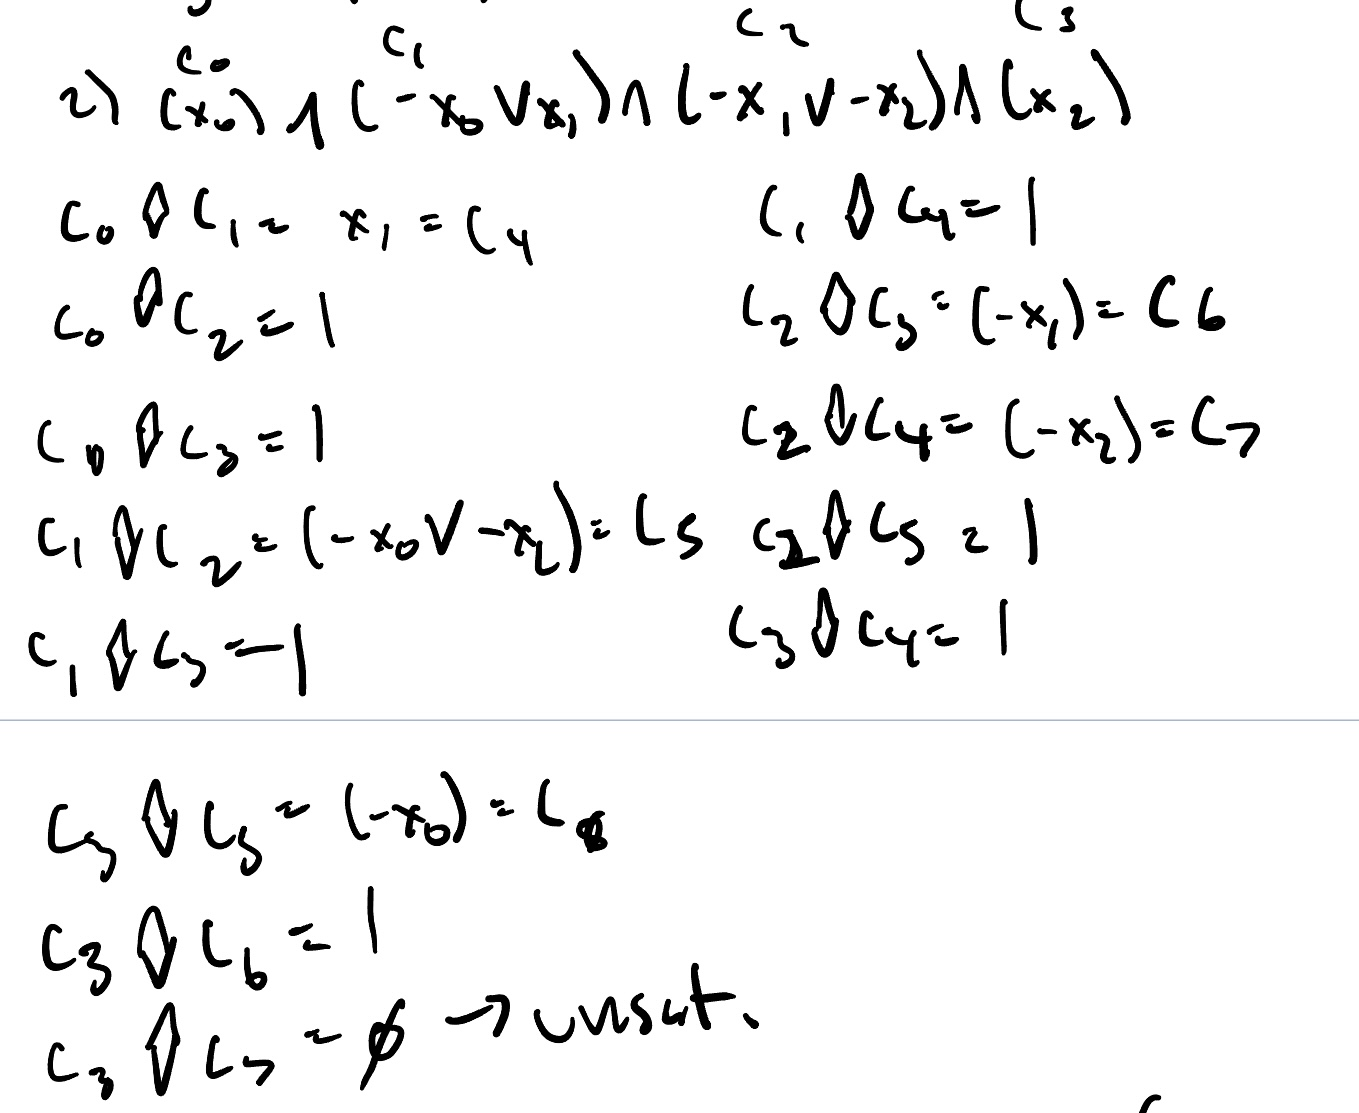
\includegraphics[width=.6\textwidth]{fall2022/psets/ps7/IMG_0017.jpg} \\
      
      Thus the problem is unsatisfiable. 
      
      
      \item $\varphi(x_0, x_1, x_2, x_3) = (x_0 \vee x_1 \vee \neg x_3) \wedge (x_2) \wedge (x_0 \vee \neg x_2) \wedge (x_1 \vee x_2)$. \\
      
      We start by defining clauses like last part. We have $C_0 =  (x_0 \vee x_1 \vee \neg x_3)$ ,$C_1 = (x_2)$, $C_2 = (x_0 \vee \neg x_2)$, $C_3 = (x_1 \vee x_2)$. Then, we proceed with ResolutionInOrder and obtain: \\
      
      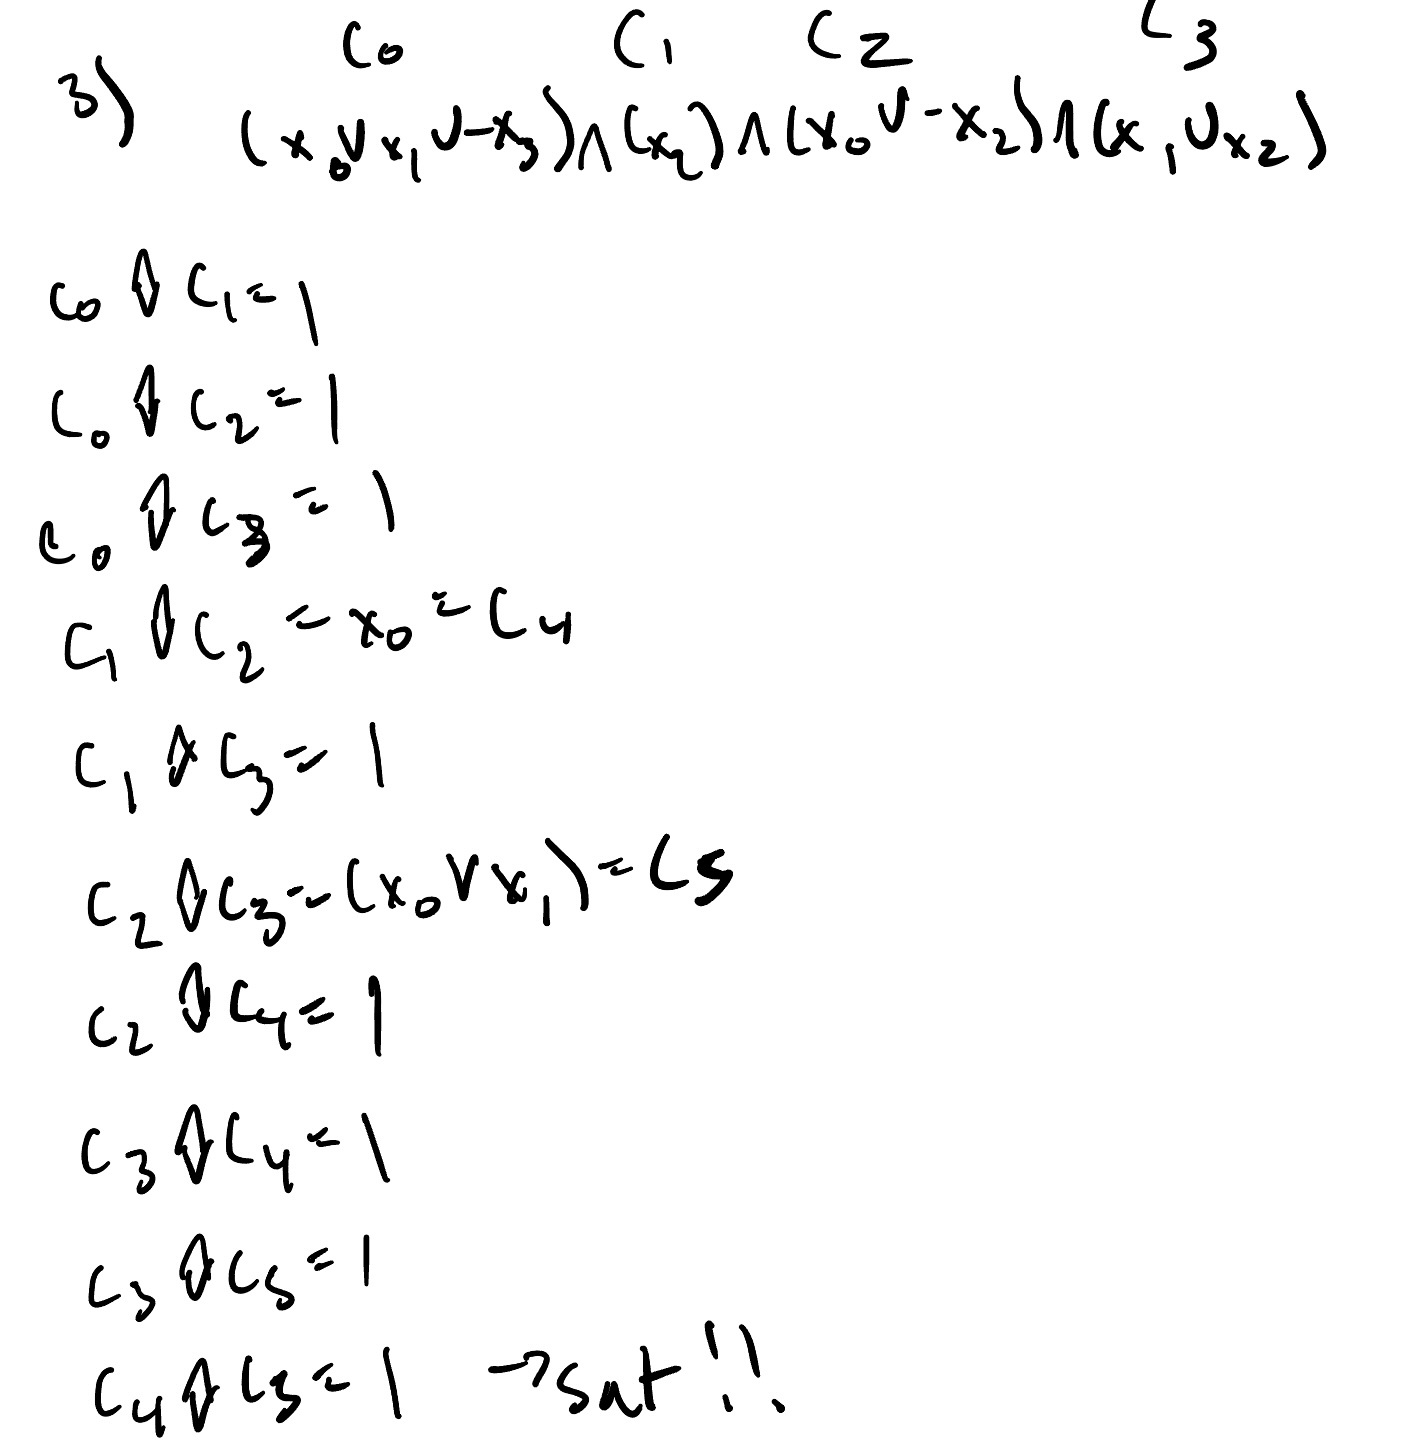
\includegraphics[width=.6\textwidth]{fall2022/psets/ps7/IMG_0018.jpg} \\
      
      Now since we determined the problem is satisfiable using ResolutionInOrder, we must identify a satisfiable solution using ExtractAssignment. We set 
      $$
      C = (x_0 \vee x_1 \vee \neg x_3) \wedge (x_2) \wedge (x_0 \vee \neg x_2) \wedge (x_1 \vee x_2) \wedge (x_0) \wedge (x_0 \vee x_v1).
      $$
      
      Now, we proceed by checking through each variable consecutively and resolving clauses. We first start with $x_0$. Since $(x_0) \in C$, we set $\alpha_0 = 1$, and resolve all clauses with $x_0$. We update $C$. Thus, we now have 
      $$
      C = (1 \vee x_1 \vee \neg x_3) \wedge (x_2) \wedge (1 \vee \neg x_2) \wedge (x_1 \vee x_2) \wedge (1) \wedge (1 \vee x_v1)
      $$
      $$
       = 1 \wedge (x_2) \wedge 1 \wedge (x_1 \vee x_2) \wedge 1 \wedge 1
      $$
      
      Now we proceed to check $x_1$. Since $(x_1) \notin C$, we set $a_1 = 0$ and resolve unresolved clauses. Thus, we have 
      $$
      C = 1 \wedge (x_2) \wedge 1 \wedge (0 \vee x_2) \wedge 1 \wedge 1
      $$
      $$
      C = 1 \wedge (x_2) \wedge 1 \wedge (0 \vee x_2) \wedge 1 \wedge 1
      $$
      Now, we check $x_2$. Since $(x_2) \in C$, we resolve. We set $a_2 = 1$, and have
      $$
      C = 1 \wedge 1 \wedge 1 \wedge 1 \wedge 1 \wedge 1 = 1
      $$
      Then, we proceed to check $x_3$. Since $(x_3) \notin C$, we simply set $x_3 = 0$. We have then determined a value for all variables that satisfies the clauses. Our solution is $$
      \alpha = \{x_0, x_1, x_2, x_3\} = \{1, 0, 1, 0\}
      $$
  \end{enumerate}
  
\item (Reductions to SAT)  Consider the following problem.  From Harvard's $n$ CS concentrators (e.g. $n=400$), we want to form a team of exactly $k$ students (e.g. $k=30$) to represent Harvard in a new programming competition.  The programming competition problems may require expertise in any of $m$ different programming languages (e.g. $m=100$).  But each of the CS concentrators only knows a few different programming languages, with a different set per person. So we want to try to find $k$ Harvard CS concentrators such that between them, they know all $m$ languages. Formally, we want to solve the following computational problem:

\compprob{ProgrammingTeam()}
{A finite set $L=\{\ell_0,\ldots,\ell_{m-1}\}$ of programming languages; a finite set 
$S=\{s_0,\ldots,s_{n-1}\}$ of students; for each student $s\in S$, a set $K(s)\subseteq L$ of languages that student $s$ knows; and a team size $k\in \N$}
{A team $T\subseteq S$ of size $k$ that collectively knows all of the programming languages in $L$ (i.e. $\bigcup_{s\in T} K(s)=L$), if one exists}

\begin{enumerate}
    \item 
Show that ProgrammingTeam can be efficiently reduced to solving a SAT instance on $kn$ variables and $m+O(kn^2)$ clauses.  Prove the correctness of your reduction and analyze its runtime.\\

Preprocess:
Since we want to use $kn$ variables total, we can think of using $k$ variables per student. Thus, let $u_{0, 0}, \cdots, u_{k-1, 0}$ be the variables representing which position the team student $0$ occupies. That is, if $u_{i, 0} = 1$ then student $0$ would occupy the $i^{th}$ place on the team. Thus, we would have $u_{0, 0} \cdots u_{k-1, n-1}$ variables total. \\

Now, we need a clause for every programming language, as we want them all to be contained within the knowledge space of the students on the team. Thus, for each language $l_0, l_1, \cdots, l_{m-1}$ we defined a clause. For some $l_i$, we define a clause $c_i$ such that $\forall$ $s_0, s_1, \cdots s_p$, we have $l_i \in K(s_j)$ where $j=0, 1, \cdots p$. That is, we want to select all the students that contain $l_i$ in their knowledge space $K(s)$. We said for an arbitrary language $l_i$ where $i=0, 1, \cdots m-1$, let those students be $s_0, s_1, \cdots s_p$ for the language. Then, we create the clause $c_i$ by including all the $u$ literals/variables associated with each $s_j \in \{s_0, s_1, \cdots, s_p\}$. Thus, we form the clause $c_i$ by letting 
$$
c_i = (u_{0, 0} \vee \cdots \vee u_{k-1, 0}, u_{0, 1} \vee \cdots \vee u_{k-1, 1}, \cdots, u_{0, p} \vee \cdots \vee u_{k-1, p},)
$$
for which the clauses we want to solve together are 
$$
c_0 \wedge c_1 \wedge \cdots \wedge c_{m-1}.
$$

Importantly, however, we must add more clauses, because we don't want to allow two students to occupy the same location on the team. That is, for every $i=0, 1, \cdots, k-1$, for every pair $(j, k)$ where both $j, k \in \{0, 1, \cdots, n-1\} : j \neq k$, we add the clause 
$$w_q = \neg u_{i, j} \vee \neg u_{i, k}.$$
We would have $q = 0, 1, \cdots O(kn^2) - 1$ w's, or extra clauses and also need to solve
$$w_0, w_1, \cdots, w_{O(kn^2) - 1}.$$ 

Now we must add clauses to ensure that no student occupies multiple locations on the team. Thus, we must add extra clauses such that for every $i=0, 1, \cdots n$ and every $y, z = 0, 1, \cdots k-1 : y \neq z$, we add a clause $d = (\neg u_{y, i} \vee \neg u_{z, i})$. Thus, we end up adding clauses $d_0 \cdots d_{O(k^2n)}$ since for every student we must go through all positions of the team to ensure they don't overlap. 

Finally, we must add $k$ clauses to ensure that all spots on the team are filled. Thus, we add clauses such as $(u_{0, 0} 
\vee u_{0, 1} \vee \cdots u_{0, n-1}) \wedge \cdots \wedge (u_{k-1, 0} \vee u_{k-1, 1} \vee \cdots u_{k-1, n-1})$. \\

Thus, we have $kn$ variables $u_{0, 0} \cdots u_{k-1, n-1}$ and must solve clauses $c_0 \wedge \cdots \wedge c_{m-1} \wedge w_0 \wedge \cdots \wedge w_{O(kn^2) - 1} \wedge d_0 \wedge \cdots \wedge d_{O(k^2n)}$ along with the extra clauses to make sure all team spots are occupied at the end as defined above. \\
Oracle: We call the SAT solver oracle so solve the SAT problem defined above. \\
Post-process: Once we have the list of solutions $\alpha = \{u_{0, 0}, \cdots, u_{k-1, n-1}\}$ where some are equal to 0 and others are equal to 1, we post-process by, for every $u_{a, b}$ where $a=0, 1, \cdots k-1$ and $b=0, 1, \cdots n-1$ where $u_{a, b} = 1$, we assign student $s_b$ to the team. Since the clauses defined in the reduction limit the number of such variables $u$ to $k$, we will have found a solution to the ProgrammingTeam problem, and have successfully completed the reduction. \\
\\ Now we must prove correctness of the reduction. First, suppose there is no solution. Then we want the output of the reduction to be $\bot$. Note that the meaning of no solution in the context of ProgrammingTeam is that there exist at least some language $l_i$ such that $l_i \notin K(s_0) \cup K(s_1) \cup \cdots \cup K(s_{n-1})$. Now consider the reduction. In the reduction, after pre-processing, we create a clause for every language in which the literals of the clause are all $u_{0, j} \cdots u_{k-1, j}$ for all $j=0, \cdots n-1$ such that $l \in K(s_j)$. However, for the particular $l_i$ we identified, there are no such $s_j$, thus there are no literals that can evaluate to True (1) to make the clause True. Thus, there is no solution, and the reduction too outputs $\bot$. \\

Now we must check that the algorithm for the reduction indeed finds a solution if it exists. In the pre-processing step, we encode the ProgrammingTeam problem into the variables and clauses we need to provide as input to the SAT solver oracle. If we have a solution, then we must satisfy $c_0 \wedge \cdots \wedge c_{m-1}$ where $c_i$ is defined as within the reduction. Within the pre-processing step, we create $k$ variables for each student. Note that for the way we implemented the pre-processing, for any language $l_i$ and corresponding clause $c_i$ and for a particular student $s_j$ where $j=0, 1, \cdots, n-1$, if $l_i \in K(s_j)$, that is, if student $j$ knows language $l_i$, then we add all its variables $u_{0, j} \cdots u_{k-1, j}$ to the clause $c_i$. Furthermore, if $l_i \notin K(s_j)$, then we do not add $u_{0, j} \cdots u_{k-1, j}$ to the clause. Thus, when we want to solve $c_0 \wedge \cdots c_{m-1}$, we can guarantee that the literals/variables contained within each clause correspond to the variables that are actually know each programming language. Furthermore, the pre-processing step to add the clauses $w_0 \cdots w_{O(kn^2)}$ as defined within the definition of the reduction algorithm ensures that no two students can have the same place on the team when we use $kn$ variables. Meanwhile, we have that the clauses $d_0 \cdots d_{O(k^2n)}$ as defined in the preprocessing step ensure that no student occupies multiple slots on the team, while the final step of the preprocessing ensures that all team spots sare occupied to build a team of size $k$. Next, we can ensure that the SAT solver oracle correctly solves the clauses we provide after pre-processing to output a valid solution $\alpha = \{u_{0, 0} \cdots u_{k-1, n-1}\}$, where $k$ such variables are $1$. Then in the post processing step, we make sure to only select the variables that are equal to $1$, or are True. In the post-processing step, we take all these such variables and include the students corresponding to each variable that is True, as we already defined. Thus, we successfully constructed the team and have correctly solved the ProgrammingTeam problem via reduction to the SAT solving problem. \\

The runtime of this algorithm can be calculated by considering the preprocessing, oracle call, and postprocessing step. The preprocessing step involves the creation of the actual clauses themselves. In particular, we noted that we created clauses $c_0, \cdots, c_{m-1}$ to satisfy each language requirement, and $O(kn^2)$ extra clauses $w_0, \cdots w_{O(kn^2)}$ to satisfy the extra clauses that prevents two students from taking the same seat on the team. Note that in creating the $m$ clauses, we must check through every student to see if we include them in the clause. Thus, the runtime of this portion is $O(knm)$, whereas the creating $O(kn^2)$ clauses has constant runtime at each step -> we just go through all combination pairs for students on the team and prevent the same spot from being taken by adding a clause containing those $2$ variables. Additionally, the next step to ensure no student occupies multiple spaces contains $O(k^2n)$ clauses, which we can most likely assume to be $O(kn^2)$ since we can consider forming each clause as $O(1)$, and because $n$ is likely greater than $k$, as the team can only be as big as the number of students. Finally, the last step to make sure all spots are occupied on the team adds only $k$ clauses and is therfore $O(k)$. Thus, the overall runtime of preprocessing is $O(knm + kn^2 + k^2n + k) = O(knm + kn^2)$ (If we assume $n > k$. The runtime of the oracle call step is simply the runtime of the fastest SAT solver, which is estimated at an exponential $O(1.33^n)$. Finally, for post-processing, we simply check through the list of $kn$ values and wherever equal to $1$, we add the corresponding student to the team. Thus, because we have $kn$ variables to check through, the runtime of the postprocessing step is simply $O(kn)$. Thus, the overall runtime of the entire reduction is $O(kmn + kn^2 + 1.33^n)$, meaning the algorithm speed is most likely dominated by the exponential term and the number of students, $n$. 


\item 
(optional\footnotemark[1])
Come up with a more efficient reduction that produces a SAT instance with $O(kn)$ variables and $m+O(kn)$ clauses (or even $m+O(n\log k)$ clauses). (Hint: something like $\psi_{n,k}$ or $\tau_\ell$ formulas from the Section 7 problem on IndependentSet$\leq$ SAT might be useful.)
\end{enumerate}
 
\end{enumerate}


\end{document}
